\documentclass[tikz]{standalone}
\usepackage{pgfplots}
\pgfplotsset{compat=1.15}
\usepackage{mathrsfs}
\usetikzlibrary{arrows,calc}
\usepackage{tkz-euclide}
\pagestyle{empty}

\definecolor{AngleClr}{rgb}{0,0.39215686274509803,0}
\definecolor{ShapeClr}{rgb}{0.6,0.2,0}

\begin{document}

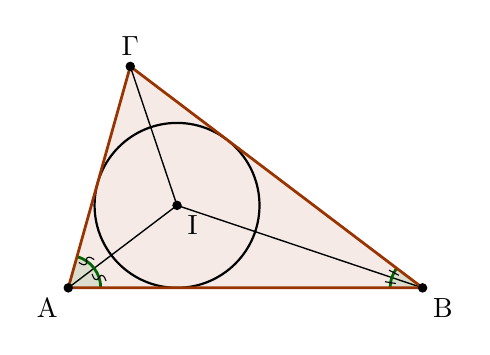
\begin{tikzpicture}[scale=.75]
\tkzSetUpLine[line width=1pt,color=black]
\tkzSetUpPoint[fill=black]

\tkzDefPoints{0/0/A,6/0/B,1.05/3.75/C}

\tkzInCenter(A,B,C)\tkzGetPoint{I}
\tkzDefPointBy[projection=onto A--B](I)\tkzGetPoint{IC}
\tkzDefPointBy[projection=onto B--C](I)\tkzGetPoint{IA}
\tkzDefPointBy[projection=onto A--C](I)\tkzGetPoint{IB}

\tkzFillPolygon[fill=ShapeClr,fill opacity=0.1,inner sep=1cm](A,B,C)

\tkzDrawSegments[line width=0.5pt,color=black](A,I B,I C,I)

\tkzFillAngles[fill=AngleClr,size=.55,fill opacity=0.1](I,B,A C,B,I)
\tkzMarkAngles[mark=|,mksize=2,line width=1pt,size=.55,color=AngleClr](I,B,A C,B,I)

\tkzFillAngles[fill=AngleClr,size=.55,fill opacity=0.1](B,A,I I,A,C)
\tkzMarkAngles[mark=s,mksize=2,line width=1pt,size=.55,color=AngleClr](B,A,I I,A,C)

\tkzDrawCircle[line width=0.8pt, black](I,IA)

\tkzDrawPolygon[color=ShapeClr](A,B,C)
\tkzDrawPoints[size=3](A,B,C,I)
\tkzLabelPoint[below left](A){$\mathrm{A}$}
\tkzLabelPoint[below right](B){$\mathrm{B}$}
\tkzLabelPoint[above](C){$\mathrm{\Gamma}$}
\tkzLabelPoint[below right](I){$\mathrm{I}$}

\end{tikzpicture}
\end{document}
